% Options for packages loaded elsewhere
\PassOptionsToPackage{unicode}{hyperref}
\PassOptionsToPackage{hyphens}{url}
%
\documentclass[
]{article}
\usepackage{lmodern}
\usepackage{amssymb,amsmath}
\usepackage{ifxetex,ifluatex}
\ifnum 0\ifxetex 1\fi\ifluatex 1\fi=0 % if pdftex
  \usepackage[T1]{fontenc}
  \usepackage[utf8]{inputenc}
  \usepackage{textcomp} % provide euro and other symbols
\else % if luatex or xetex
  \usepackage{unicode-math}
  \defaultfontfeatures{Scale=MatchLowercase}
  \defaultfontfeatures[\rmfamily]{Ligatures=TeX,Scale=1}
\fi
% Use upquote if available, for straight quotes in verbatim environments
\IfFileExists{upquote.sty}{\usepackage{upquote}}{}
\IfFileExists{microtype.sty}{% use microtype if available
  \usepackage[]{microtype}
  \UseMicrotypeSet[protrusion]{basicmath} % disable protrusion for tt fonts
}{}
\makeatletter
\@ifundefined{KOMAClassName}{% if non-KOMA class
  \IfFileExists{parskip.sty}{%
    \usepackage{parskip}
  }{% else
    \setlength{\parindent}{0pt}
    \setlength{\parskip}{6pt plus 2pt minus 1pt}}
}{% if KOMA class
  \KOMAoptions{parskip=half}}
\makeatother
\usepackage{xcolor}
\IfFileExists{xurl.sty}{\usepackage{xurl}}{} % add URL line breaks if available
\IfFileExists{bookmark.sty}{\usepackage{bookmark}}{\usepackage{hyperref}}
\hypersetup{
  pdftitle={Simplified Template for DSI AT2},
  pdfauthor={Peter Kiel modified by Simon Knight and Durand Sinclair},
  hidelinks,
  pdfcreator={LaTeX via pandoc}}
\urlstyle{same} % disable monospaced font for URLs
\usepackage[margin=1in]{geometry}
\usepackage{color}
\usepackage{fancyvrb}
\newcommand{\VerbBar}{|}
\newcommand{\VERB}{\Verb[commandchars=\\\{\}]}
\DefineVerbatimEnvironment{Highlighting}{Verbatim}{commandchars=\\\{\}}
% Add ',fontsize=\small' for more characters per line
\usepackage{framed}
\definecolor{shadecolor}{RGB}{248,248,248}
\newenvironment{Shaded}{\begin{snugshade}}{\end{snugshade}}
\newcommand{\AlertTok}[1]{\textcolor[rgb]{0.94,0.16,0.16}{#1}}
\newcommand{\AnnotationTok}[1]{\textcolor[rgb]{0.56,0.35,0.01}{\textbf{\textit{#1}}}}
\newcommand{\AttributeTok}[1]{\textcolor[rgb]{0.77,0.63,0.00}{#1}}
\newcommand{\BaseNTok}[1]{\textcolor[rgb]{0.00,0.00,0.81}{#1}}
\newcommand{\BuiltInTok}[1]{#1}
\newcommand{\CharTok}[1]{\textcolor[rgb]{0.31,0.60,0.02}{#1}}
\newcommand{\CommentTok}[1]{\textcolor[rgb]{0.56,0.35,0.01}{\textit{#1}}}
\newcommand{\CommentVarTok}[1]{\textcolor[rgb]{0.56,0.35,0.01}{\textbf{\textit{#1}}}}
\newcommand{\ConstantTok}[1]{\textcolor[rgb]{0.00,0.00,0.00}{#1}}
\newcommand{\ControlFlowTok}[1]{\textcolor[rgb]{0.13,0.29,0.53}{\textbf{#1}}}
\newcommand{\DataTypeTok}[1]{\textcolor[rgb]{0.13,0.29,0.53}{#1}}
\newcommand{\DecValTok}[1]{\textcolor[rgb]{0.00,0.00,0.81}{#1}}
\newcommand{\DocumentationTok}[1]{\textcolor[rgb]{0.56,0.35,0.01}{\textbf{\textit{#1}}}}
\newcommand{\ErrorTok}[1]{\textcolor[rgb]{0.64,0.00,0.00}{\textbf{#1}}}
\newcommand{\ExtensionTok}[1]{#1}
\newcommand{\FloatTok}[1]{\textcolor[rgb]{0.00,0.00,0.81}{#1}}
\newcommand{\FunctionTok}[1]{\textcolor[rgb]{0.00,0.00,0.00}{#1}}
\newcommand{\ImportTok}[1]{#1}
\newcommand{\InformationTok}[1]{\textcolor[rgb]{0.56,0.35,0.01}{\textbf{\textit{#1}}}}
\newcommand{\KeywordTok}[1]{\textcolor[rgb]{0.13,0.29,0.53}{\textbf{#1}}}
\newcommand{\NormalTok}[1]{#1}
\newcommand{\OperatorTok}[1]{\textcolor[rgb]{0.81,0.36,0.00}{\textbf{#1}}}
\newcommand{\OtherTok}[1]{\textcolor[rgb]{0.56,0.35,0.01}{#1}}
\newcommand{\PreprocessorTok}[1]{\textcolor[rgb]{0.56,0.35,0.01}{\textit{#1}}}
\newcommand{\RegionMarkerTok}[1]{#1}
\newcommand{\SpecialCharTok}[1]{\textcolor[rgb]{0.00,0.00,0.00}{#1}}
\newcommand{\SpecialStringTok}[1]{\textcolor[rgb]{0.31,0.60,0.02}{#1}}
\newcommand{\StringTok}[1]{\textcolor[rgb]{0.31,0.60,0.02}{#1}}
\newcommand{\VariableTok}[1]{\textcolor[rgb]{0.00,0.00,0.00}{#1}}
\newcommand{\VerbatimStringTok}[1]{\textcolor[rgb]{0.31,0.60,0.02}{#1}}
\newcommand{\WarningTok}[1]{\textcolor[rgb]{0.56,0.35,0.01}{\textbf{\textit{#1}}}}
\usepackage{longtable,booktabs}
% Correct order of tables after \paragraph or \subparagraph
\usepackage{etoolbox}
\makeatletter
\patchcmd\longtable{\par}{\if@noskipsec\mbox{}\fi\par}{}{}
\makeatother
% Allow footnotes in longtable head/foot
\IfFileExists{footnotehyper.sty}{\usepackage{footnotehyper}}{\usepackage{footnote}}
\makesavenoteenv{longtable}
\usepackage{graphicx,grffile}
\makeatletter
\def\maxwidth{\ifdim\Gin@nat@width>\linewidth\linewidth\else\Gin@nat@width\fi}
\def\maxheight{\ifdim\Gin@nat@height>\textheight\textheight\else\Gin@nat@height\fi}
\makeatother
% Scale images if necessary, so that they will not overflow the page
% margins by default, and it is still possible to overwrite the defaults
% using explicit options in \includegraphics[width, height, ...]{}
\setkeys{Gin}{width=\maxwidth,height=\maxheight,keepaspectratio}
% Set default figure placement to htbp
\makeatletter
\def\fps@figure{htbp}
\makeatother
\setlength{\emergencystretch}{3em} % prevent overfull lines
\providecommand{\tightlist}{%
  \setlength{\itemsep}{0pt}\setlength{\parskip}{0pt}}
\setcounter{secnumdepth}{5}

\title{Simplified Template for DSI AT2}
\usepackage{etoolbox}
\makeatletter
\providecommand{\subtitle}[1]{% add subtitle to \maketitle
  \apptocmd{\@title}{\par {\large #1 \par}}{}{}
}
\makeatother
\subtitle{Enter your student ID here}
\author{Peter Kiel modified by Simon Knight and Durand Sinclair}
\date{22/08/2019}

\begin{document}
\maketitle

{
\setcounter{tocdepth}{2}
\tableofcontents
}
\begin{center}\rule{0.5\linewidth}{0.5pt}\end{center}

\hypertarget{preface-how-to-use-this-guide}{%
\subsection{Preface: How to use this
guide}\label{preface-how-to-use-this-guide}}

This document has a suggested structure for your report, starting from
section 1 ``Introduction''. Before that, we have some tutorials on how
to set up your environment, which you can delete once you've read so you
don't hand them in.

The basic structure of this template is similar to the style of academic
papers and, if followed, should ensure that everything you need to
include is present. I have included the assessment criteria at the
relevant places to remind you of what needs to be in the report.

You are free to vary the structure by renaming the sections, including
other sections, or dropping ones that you don't use. Keep in mind that
the suggested structure is conventional (and therefore easy to follow),
practical, and comprehensive. (Criterion 5: Professionally presented in
a manner appropriate to the discipline.) If you do use this template,
you will need to install R, RStudio, and the packages listed in the code
block at the head of this document.

Note: We have provided some sample code below, along with some text
between angle brackets, \textless{} \textgreater. All of this should be
replaced by your work.

\textbf{\emph{Please don't forget to include a title, name, student
number, etc. on a covering sheet}}

\hypertarget{set-up-a-project}{%
\subsection{Set up a project}\label{set-up-a-project}}

It is best to set up your assignment as a project, rather than just have
a single RMarkdown file. Setting up a project will define your working
directory based on where a .RProj file is located. Other files and
folders can then be found relative to that .RProj file. This gives
projects some advantages: - It's easier to find your files, because you
can set up subfolders with consistent names - You can refer to your data
with relative referencing, eg \texttt{data/my\_data.csv}, rather than
having to type
\texttt{C:\textbackslash{}folder\textbackslash{}other\_folder\textbackslash{}data\textbackslash{}my\_data.csv}.
- When you open your project, it unloads your libraries and clears your
memory. That way, the libraries that you had loaded before won't get in
the way of the one you're working on now. But when you close this
project, it goes back to the state it was in before.

To start a project in RStudio, - click File -\textgreater{} New Project
and follow the prompts to set up a new project in a new folder. - Create
subfolders called ``R'' and ``data''. - Save this template to the R
folder, along with any other R code files you create on the project. -
Save any data files (eg csv files, or screenshots from your other
analysis) to the data folder.

I highly recommend
\href{\%22https://www.tidyverse.org/articles/2017/12/workflow-vs-script/\%22}{this
link on project-oriented workflow}

\hypertarget{install-packages}{%
\subsection{Install packages}\label{install-packages}}

If we don't have these packages, we'll need to download them from the
internet. Here's some code that does that. The code is currently
commented out (that is, it has a ``\#'' at the start of the line.)
Remove the ``\#'' if you want to install those packages.

\begin{Shaded}
\begin{Highlighting}[]
\CommentTok{# install.packages(c("tidyverse", "here", "knitr"))}

\CommentTok{# devtools::install_github("benmarwick/wordcountaddin", }
\CommentTok{#                         type = "source", }
\CommentTok{#                         dependencies = TRUE)}

\CommentTok{## Go to Tools > Addins > Browse Addins, and then search for wordcountaddin. }
\CommentTok{## There will be two. Click them one at a time and click the Execute button. }
\end{Highlighting}
\end{Shaded}

Now, test the file by using the `knit' button (just above this code
chunk). Read more about R markdown and `kniting' (rendering) documents
here:
\url{https://rmarkdown.rstudio.com/authoring_quick_tour.html\#overview}

Installing the packages only puts them on our computer. To use them in
our project, we need them loaded.

\begin{Shaded}
\begin{Highlighting}[]
  \CommentTok{# Load libraries}
  \KeywordTok{library}\NormalTok{(psych)}
  \KeywordTok{library}\NormalTok{(devtools)}

  \KeywordTok{library}\NormalTok{(tidyverse)}
  \KeywordTok{library}\NormalTok{(here)}
  
  \KeywordTok{library}\NormalTok{(knitr)}
  \KeywordTok{library}\NormalTok{(kfigr) }\CommentTok{#this lets us crossreference figures, etc. Read more about it }
                \CommentTok{#at https://github.com/mkoohafkan/kfigr/edit/master/vignettes/introduction.Rmd }
\end{Highlighting}
\end{Shaded}

\hypertarget{calculating-word-length}{%
\subsection{Calculating word length}\label{calculating-word-length}}

The word limit is 2800 words (excluding data excerpts and appendices,
visualisations, and references) To check this, you can either copy the
html output to word, or use the addin Word Count Addin. E.g.
\texttt{wordcountaddin:::text\_stats()}

\begin{longtable}[]{@{}lll@{}}
\toprule
Method & koRpus & stringi\tabularnewline
\midrule
\endhead
Word count & 436 & 427\tabularnewline
Character count & 2624 & 2609\tabularnewline
Sentence count & 25 & Not available\tabularnewline
Reading time & 2.2 minutes & 2.1 minutes\tabularnewline
\bottomrule
\end{longtable}

\hypertarget{citations}{%
\subsection{Citations}\label{citations}}

In this assignment, we'll use footnotes to do citation. Here's how to do
it. \footnote{This is the text of the footnote which you can see at the
  bottom of the page.}

\hypertarget{formatting-guide}{%
\subsection{Formatting guide}\label{formatting-guide}}

Here are some formatting tricks you can use.

\hypertarget{fonts}{%
\subsubsection{Fonts}\label{fonts}}

\emph{italics}\\
\textbf{bold}\\
\textbf{\emph{bold italics}}\\
\texttt{verbatim\ code}~\\
superscript\textsuperscript{2}\\
subscript\textsubscript{2}

\begin{quote}
This is a block quotation, if you have a long quote from someone this is
the best way to do it (but don't forget the citation). This is a very
long line that will still be quoted properly when it wraps. Oh boy let's
keep writing to make sure this is long enough to actually wrap for
everyone. Oh, you can \emph{put} \textbf{Markdown} into a blockquote.
\end{quote}

\hypertarget{headings}{%
\subsubsection{Headings}\label{headings}}

Add headings using a \# (but note, to get that to display properly I had
to `escape' it using a preceding backslash). One \# gives you a line
with Heading 1 style, \#\# gives you Heading 2 etc.

\hypertarget{lists}{%
\subsubsection{Lists}\label{lists}}

\begin{enumerate}
\def\labelenumi{\arabic{enumi}.}
\tightlist
\item
  Numbered
\item
  Lists
\item
  Are
\item
  Possible
\end{enumerate}

\begin{itemize}
\tightlist
\item
  And so
\item
  are bulleted lists
\end{itemize}

More examples can be found
\href{https://www.rstudio.com/wp-content/uploads/2016/03/rmarkdown-cheatsheet-2.0.pdf}{on
the cheat sheet at this hyperlink}

\hypertarget{equations}{%
\subsubsection{Equations}\label{equations}}

If you want to insert equations (you probably don't) you can do so using
the syntax below. You can also insert bits of inline code like, so the
\texttt{2+2} here is produced by a piece of code, and the 4 is produced
by an equation (namely \texttt{2+2})

The deterministic part of the model is defined by this \textbf{in-line
equation} as \(\mu_i = \beta_0 + \beta_1x\), and the stochastic part by
the \textbf{centered equation}:

\[ \frac{1}{\sqrt{2\pi}\sigma}e^{-(x-\mu_i)^2/(2\sigma^2)} \] More
examples at
\href{https://www.statpower.net/Content/310/R\%20Stuff/SampleMarkdown.html}{this
hyperlink}

\hypertarget{embedding-an-image}{%
\subsection{Embedding an image}\label{embedding-an-image}}

You might have saved some analysis from another program as a picture
file. This is how you paste it: Let's embed a UTS logo, which I've saved
to the \texttt{data} folder.


\includegraphics[width=16.67in]{C:/Users/125295/Google Drive/teaching/MDSI/DSI/1 Materials for Canvas/Canvas materials/Assessment materials/AT2/AT2 template and sample/AT2 template and sample/AT2_simplified-master/data/uts_logo}

\begin{center}\rule{0.5\linewidth}{0.5pt}\end{center}

\hypertarget{introduction}{%
\section{Introduction}\label{introduction}}

\textless{} Write a paragraph that gives an overview of what you've
done. Also, make sure to include the assignment title, your name, and
student number in rows 2 to 4 at the top of the page in RMarkdown.
\textgreater{}

\hypertarget{description-of-process-or-methods}{%
\section{Description of process or
methods}\label{description-of-process-or-methods}}

\textless this is where you give details about what you've been
collecting and how much you data have; why you choose this data to
collect; how you managed the quality and frequency of collection issues;
what you did to anonymise or de-identify the data, and how you dealt
with the storage and sharing of data within the group. Do not include a
dump of all your data here. If you wish to include examples of data (and
I think you should) then put these in an appendix to the report.\\
\emph{Criterion 1: Justifies a method to obtain data from multiple
sources, for gaining insight into a chosen problem, including analysis
of data quality issues in the individual and group data.}\textgreater{}

\hypertarget{analysis}{%
\section{Analysis}\label{analysis}}

\textless describe how you analysed your data, and how you contrasted
your data with the group's data.\\
\emph{Criterion 2: Justifies the analysis of the obtained data,
including quality issues, to draw conclusions in a professional and
engaging manner.}\textgreater{}

\hypertarget{example-analysis-get-data}{%
\subsection{Example analysis: Get
data}\label{example-analysis-get-data}}

If you downloaded the full folder, then the csv files you need are
there. You can also get your own weather data if you want.

\begin{Shaded}
\begin{Highlighting}[]
\KeywordTok{library}\NormalTok{(tidyverse)}
\KeywordTok{library}\NormalTok{(here)}

\CommentTok{# Load a csv file from our hard drive}
\NormalTok{weather_sydney <-}\StringTok{ }\KeywordTok{read_csv}\NormalTok{(here}\OperatorTok{::}\KeywordTok{here}\NormalTok{(}\StringTok{"data"}\NormalTok{, }\StringTok{"syd_weath.csv"}\NormalTok{))}
\NormalTok{weather_melbourne <-}\StringTok{ }\KeywordTok{read_csv}\NormalTok{(here}\OperatorTok{::}\KeywordTok{here}\NormalTok{(}\StringTok{"data"}\NormalTok{, }\StringTok{"mel_weath.csv"}\NormalTok{))}

\CommentTok{# Load an Excel file from our hard drive}
\NormalTok{sydney_xl <-}\StringTok{ }\NormalTok{readxl}\OperatorTok{::}\KeywordTok{read_excel}\NormalTok{(}\DataTypeTok{path =}\NormalTok{ here}\OperatorTok{::}\KeywordTok{here}\NormalTok{(}\StringTok{"data"}\NormalTok{, }\StringTok{"syd_weath.xls"}\NormalTok{))}

\CommentTok{# Simulate our own data - 5 rows and 2 columns}
\NormalTok{my_fake_data1 <-}\StringTok{ }\KeywordTok{tibble}\NormalTok{(}\DataTypeTok{first_column =} \KeywordTok{c}\NormalTok{(}\DecValTok{1}\NormalTok{, }\DecValTok{1}\NormalTok{, }\DecValTok{2}\NormalTok{, }\DecValTok{1}\NormalTok{, }\DecValTok{1}\NormalTok{),}
                        \DataTypeTok{second_column =} \KeywordTok{c}\NormalTok{(}\StringTok{"a"}\NormalTok{, }\StringTok{"b"}\NormalTok{, }\StringTok{"a"}\NormalTok{, }\StringTok{"a"}\NormalTok{, }\StringTok{"b"}\NormalTok{),}
\NormalTok{                        )}

\CommentTok{#Simulate normally distributed data}
\NormalTok{my_fake_data2 <-}\StringTok{ }\KeywordTok{tibble}\NormalTok{(}\DataTypeTok{normal_column =} \KeywordTok{rnorm}\NormalTok{(}\DataTypeTok{n =} \DecValTok{50}\NormalTok{, }\DataTypeTok{mean =} \DecValTok{0}\NormalTok{, }\DataTypeTok{sd =} \DecValTok{1}\NormalTok{),}
                        \DataTypeTok{higher_column =} \KeywordTok{rnorm}\NormalTok{(}\DataTypeTok{n =} \DecValTok{50}\NormalTok{, }\DataTypeTok{mean =} \FloatTok{0.1}\NormalTok{, }\DataTypeTok{sd =} \DecValTok{1}\NormalTok{),}
                        \DataTypeTok{lower_column =} \KeywordTok{rnorm}\NormalTok{(}\DataTypeTok{n =} \DecValTok{50}\NormalTok{, }\DataTypeTok{mean =} \FloatTok{-0.1}\NormalTok{, }\DataTypeTok{sd =} \DecValTok{1}\NormalTok{)}
\NormalTok{                        )}
\end{Highlighting}
\end{Shaded}

\hypertarget{example-analysis-explore-data}{%
\subsection{Example analysis: Explore
data}\label{example-analysis-explore-data}}

\begin{Shaded}
\begin{Highlighting}[]
\CommentTok{#Explore using base R techniques}
\KeywordTok{head}\NormalTok{(weather_sydney) }\CommentTok{# First few rows of the weather_sydney table}
\end{Highlighting}
\end{Shaded}

\begin{verbatim}
## # A tibble: 6 x 22
##      X1 date                 temp dew_pt   hum wind_spd wind_gust dir     vis
##   <dbl> <dttm>              <dbl>  <dbl> <dbl>    <dbl>     <dbl> <chr> <dbl>
## 1     1 2018-02-08 00:00:00    23     15    52     16.7        NA North    30
## 2     2 2018-02-08 00:00:00    23     15    61     16.7        NA North    NA
## 3     3 2018-02-08 00:30:00    22     15    64     13          NA NNW      NA
## 4     4 2018-02-08 01:00:00    22     15    56     11.1        NA NNW      NA
## 5     5 2018-02-08 01:00:00    22     15    64     11.1        NA NNW      NA
## 6     6 2018-02-08 01:30:00    22     15    64     13          NA North    NA
## # ... with 13 more variables: pressure <dbl>, wind_chill <lgl>,
## #   heat_index <dbl>, precip <lgl>, precip_rate <lgl>, precip_total <lgl>,
## #   cond <chr>, fog <dbl>, rain <dbl>, snow <dbl>, hail <dbl>, thunder <dbl>,
## #   tornado <dbl>
\end{verbatim}

\begin{Shaded}
\begin{Highlighting}[]
\KeywordTok{dim}\NormalTok{(weather_sydney) }\CommentTok{# Number of rows and columns}
\end{Highlighting}
\end{Shaded}

\begin{verbatim}
## [1] 2206   22
\end{verbatim}

\begin{Shaded}
\begin{Highlighting}[]
\KeywordTok{colnames}\NormalTok{(weather_sydney) }\CommentTok{#Column names}
\end{Highlighting}
\end{Shaded}

\begin{verbatim}
##  [1] "X1"           "date"         "temp"         "dew_pt"       "hum"         
##  [6] "wind_spd"     "wind_gust"    "dir"          "vis"          "pressure"    
## [11] "wind_chill"   "heat_index"   "precip"       "precip_rate"  "precip_total"
## [16] "cond"         "fog"          "rain"         "snow"         "hail"        
## [21] "thunder"      "tornado"
\end{verbatim}

\begin{Shaded}
\begin{Highlighting}[]
\CommentTok{#Explore using techniques from the tidyverse package}
\KeywordTok{glimpse}\NormalTok{(weather_sydney) }\CommentTok{# Does all of the above base R techniques, but neater}
\end{Highlighting}
\end{Shaded}

\begin{verbatim}
## Rows: 2,206
## Columns: 22
## $ X1           <dbl> 1, 2, 3, 4, 5, 6, 7, 8, 9, 10, 11, 12, 13, 14, 15, 16,...
## $ date         <dttm> 2018-02-08 00:00:00, 2018-02-08 00:00:00, 2018-02-08 ...
## $ temp         <dbl> 23, 23, 22, 22, 22, 22, 22, 22, 22, 21, 21, 21, 21, 21...
## $ dew_pt       <dbl> 15, 15, 15, 15, 15, 15, 16, 16, 15, 15, 15, 15, 15, 15...
## $ hum          <dbl> 52, 61, 64, 56, 64, 64, 60, 69, 64, 62, 68, 68, 62, 68...
## $ wind_spd     <dbl> 16.7, 16.7, 13.0, 11.1, 11.1, 13.0, 11.1, 11.1, 11.1, ...
## $ wind_gust    <dbl> NA, NA, NA, NA, NA, NA, NA, NA, NA, NA, NA, NA, NA, NA...
## $ dir          <chr> "North", "North", "NNW", "NNW", "NNW", "North", "NNW",...
## $ vis          <dbl> 30, NA, NA, NA, NA, NA, NA, NA, NA, 30, NA, NA, NA, NA...
## $ pressure     <dbl> 1020, 1020, 1020, 1020, 1020, 1019, 1020, 1019, 1019, ...
## $ wind_chill   <lgl> NA, NA, NA, NA, NA, NA, NA, NA, NA, NA, NA, NA, NA, NA...
## $ heat_index   <dbl> NA, NA, NA, NA, NA, NA, NA, NA, NA, NA, NA, NA, NA, NA...
## $ precip       <lgl> NA, NA, NA, NA, NA, NA, NA, NA, NA, NA, NA, NA, NA, NA...
## $ precip_rate  <lgl> NA, NA, NA, NA, NA, NA, NA, NA, NA, NA, NA, NA, NA, NA...
## $ precip_total <lgl> NA, NA, NA, NA, NA, NA, NA, NA, NA, NA, NA, NA, NA, NA...
## $ cond         <chr> "Partly Cloudy", "Clear", "Clear", NA, "Clear", "Clear...
## $ fog          <dbl> 0, 0, 0, 0, 0, 0, 0, 0, 0, 0, 0, 0, 0, 0, 0, 0, 0, 0, ...
## $ rain         <dbl> 0, 0, 0, 0, 0, 0, 0, 0, 0, 0, 0, 0, 0, 0, 0, 0, 0, 0, ...
## $ snow         <dbl> 0, 0, 0, 0, 0, 0, 0, 0, 0, 0, 0, 0, 0, 0, 0, 0, 0, 0, ...
## $ hail         <dbl> 0, 0, 0, 0, 0, 0, 0, 0, 0, 0, 0, 0, 0, 0, 0, 0, 0, 0, ...
## $ thunder      <dbl> 0, 0, 0, 0, 0, 0, 0, 0, 0, 0, 0, 0, 0, 0, 0, 0, 0, 0, ...
## $ tornado      <dbl> 0, 0, 0, 0, 0, 0, 0, 0, 0, 0, 0, 0, 0, 0, 0, 0, 0, 0, ...
\end{verbatim}

\begin{Shaded}
\begin{Highlighting}[]
\CommentTok{#Explore by creating histograms}
\KeywordTok{hist}\NormalTok{(weather_sydney}\OperatorTok{$}\NormalTok{temp, }\DataTypeTok{main =} \StringTok{"Sydney weather"}\NormalTok{, }\DataTypeTok{xlab =} \StringTok{"Temp"}\NormalTok{)}
\end{Highlighting}
\end{Shaded}

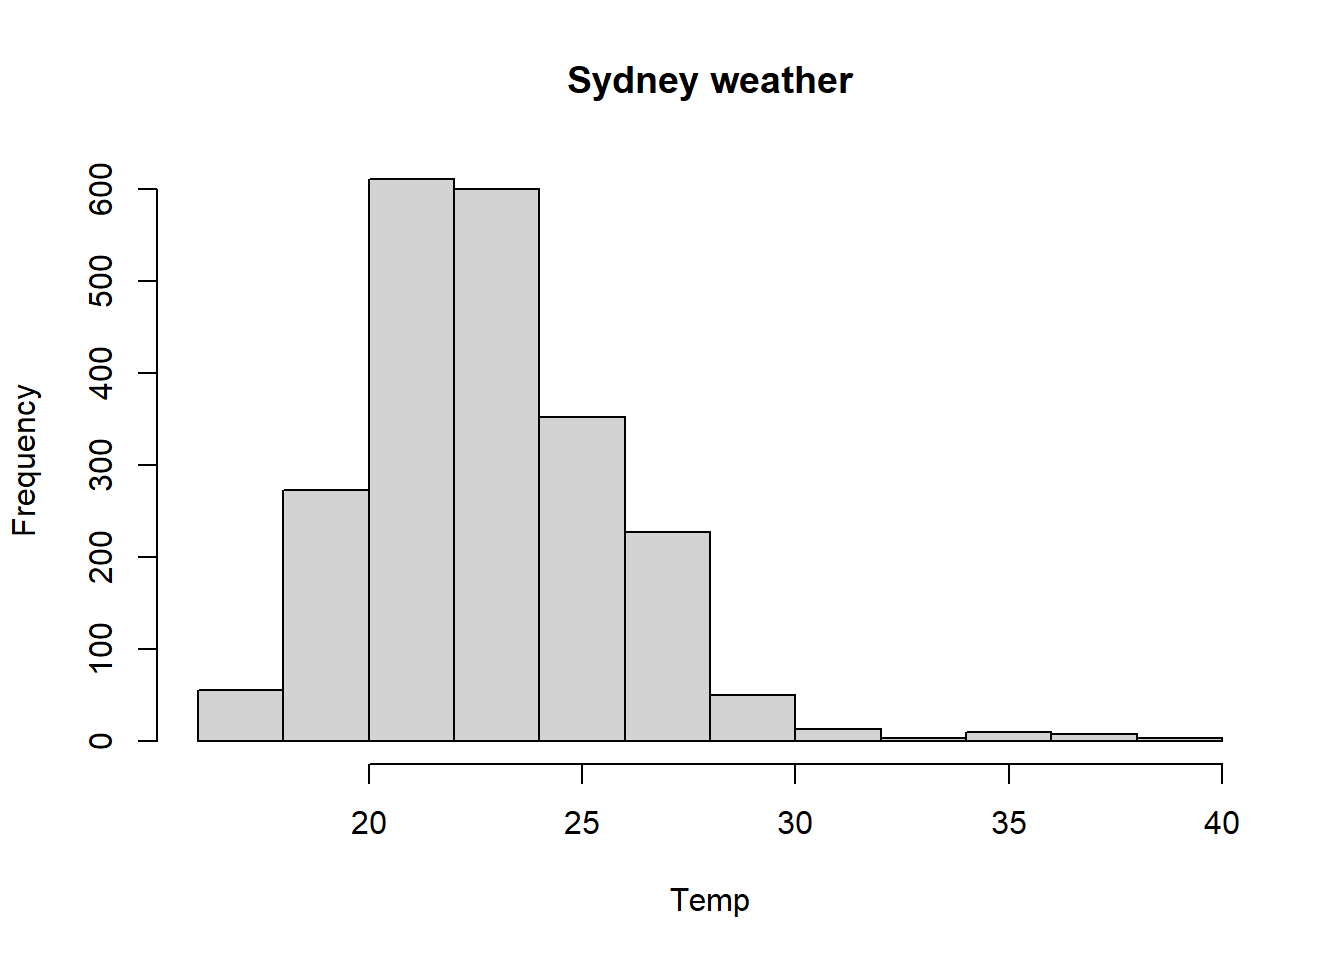
\includegraphics{template_simplified_files/figure-latex/explore_data-1.pdf}

\begin{Shaded}
\begin{Highlighting}[]
\KeywordTok{hist}\NormalTok{(weather_melbourne}\OperatorTok{$}\NormalTok{temp, }\DataTypeTok{main =} \StringTok{"Melbourne weather"}\NormalTok{, }\DataTypeTok{xlab =} \StringTok{"Temp"}\NormalTok{)}
\end{Highlighting}
\end{Shaded}

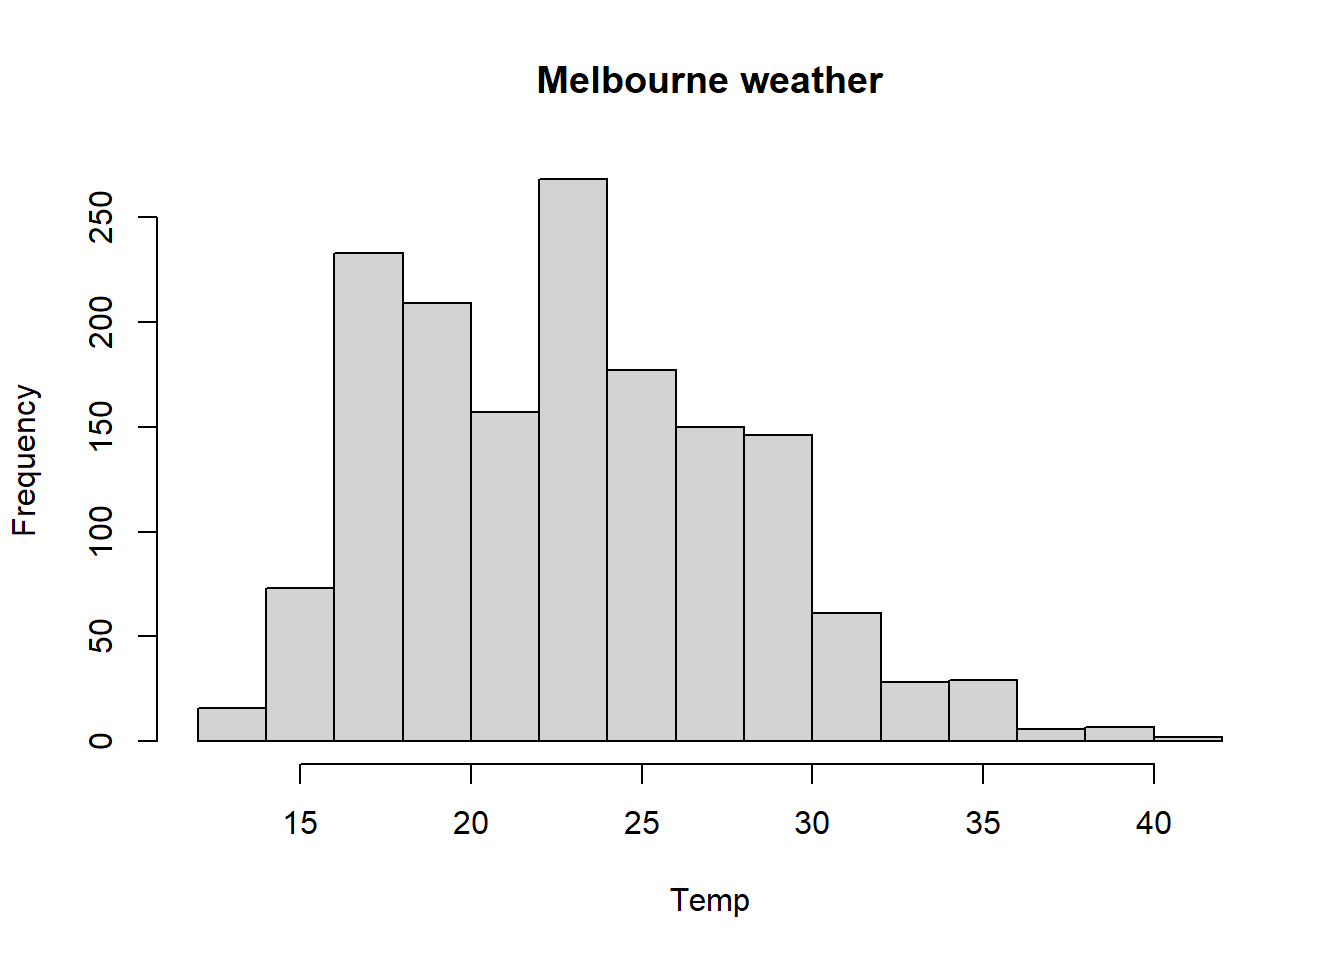
\includegraphics{template_simplified_files/figure-latex/explore_data-2.pdf}

\begin{Shaded}
\begin{Highlighting}[]
\CommentTok{#Explore by creating scatterplots}
\KeywordTok{plot}\NormalTok{(}\DataTypeTok{x =}\NormalTok{ weather_sydney}\OperatorTok{$}\NormalTok{date, }
     \DataTypeTok{y =}\NormalTok{ weather_sydney}\OperatorTok{$}\NormalTok{temp, }
     \DataTypeTok{xlab =} \StringTok{"Dates"}\NormalTok{,}
     \DataTypeTok{ylab =} \StringTok{"Temperature"}\NormalTok{,}
     \DataTypeTok{main =} \StringTok{"Sydney Temperatures in February and March"}
\NormalTok{     )}
\end{Highlighting}
\end{Shaded}

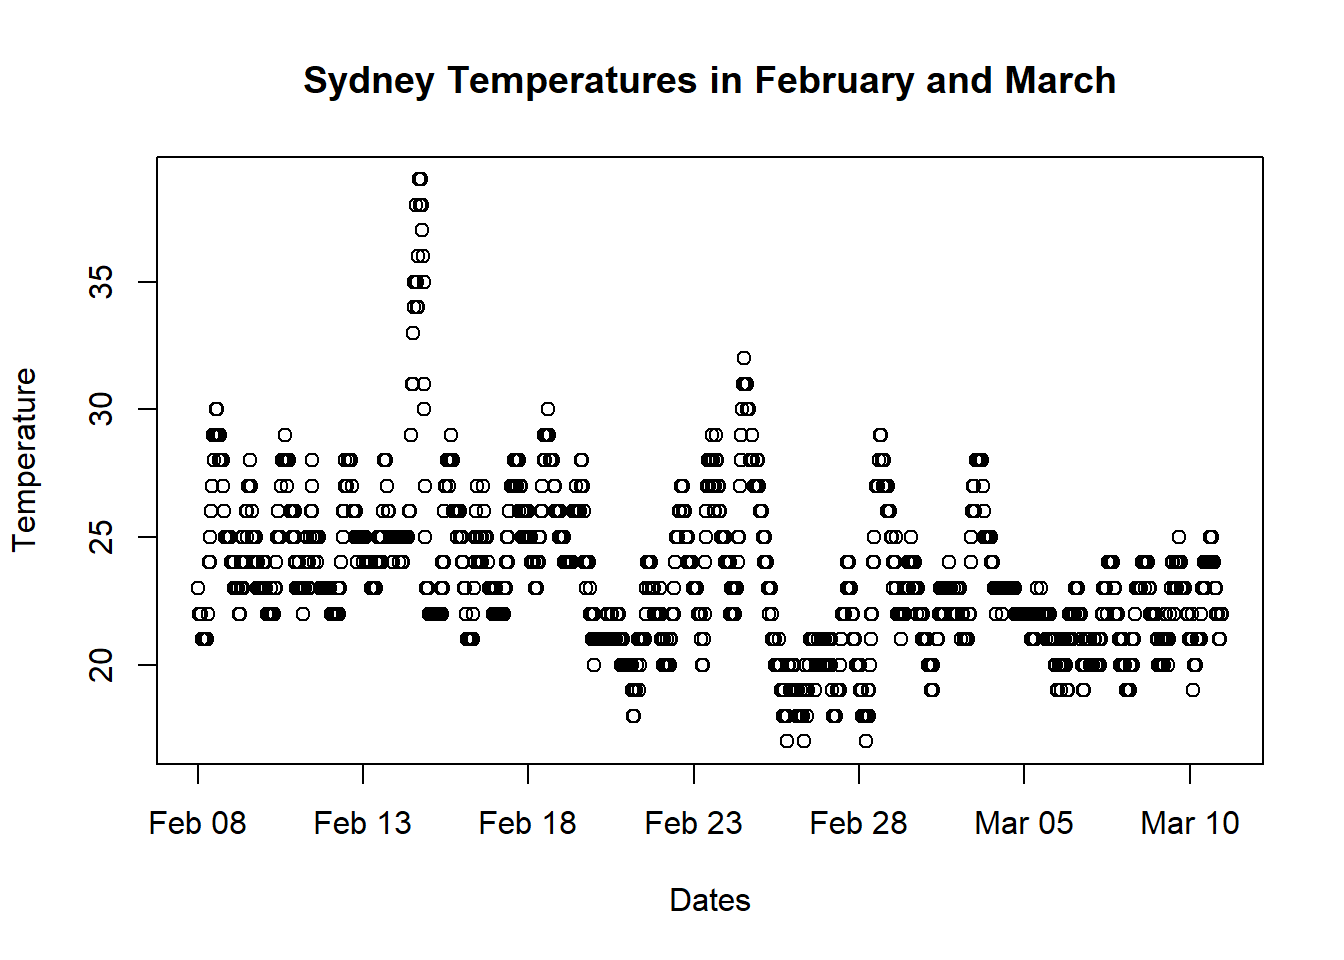
\includegraphics{template_simplified_files/figure-latex/explore_data-3.pdf}

\begin{Shaded}
\begin{Highlighting}[]
\CommentTok{#Category counts}
\KeywordTok{table}\NormalTok{(weather_sydney}\OperatorTok{$}\NormalTok{cond) }\CommentTok{# Count of each condition}
\end{Highlighting}
\end{Shaded}

\begin{verbatim}
## 
##                        Clear                      Drizzle 
##                          285                            3 
##                         Haze           Heavy Rain Showers 
##                           63                            2 
##                Light Drizzle                   Light Rain 
##                           11                           40 
##           Light Rain Showers Light Thunderstorms and Rain 
##                           72                            5 
##                Mostly Cloudy                     Overcast 
##                          591                           27 
##                Partly Cloudy                         Rain 
##                          362                           10 
##                 Rain Showers             Scattered Clouds 
##                           13                          247 
##                 Thunderstorm                      Unknown 
##                            1                            4
\end{verbatim}

\begin{Shaded}
\begin{Highlighting}[]
\KeywordTok{prop.table}\NormalTok{(}\KeywordTok{table}\NormalTok{(weather_sydney}\OperatorTok{$}\NormalTok{cond)) }\OperatorTok{*}\StringTok{ }\DecValTok{100} \CommentTok{# Percentage of each condition}
\end{Highlighting}
\end{Shaded}

\begin{verbatim}
## 
##                        Clear                      Drizzle 
##                  16.41705069                   0.17281106 
##                         Haze           Heavy Rain Showers 
##                   3.62903226                   0.11520737 
##                Light Drizzle                   Light Rain 
##                   0.63364055                   2.30414747 
##           Light Rain Showers Light Thunderstorms and Rain 
##                   4.14746544                   0.28801843 
##                Mostly Cloudy                     Overcast 
##                  34.04377880                   1.55529954 
##                Partly Cloudy                         Rain 
##                  20.85253456                   0.57603687 
##                 Rain Showers             Scattered Clouds 
##                   0.74884793                  14.22811060 
##                 Thunderstorm                      Unknown 
##                   0.05760369                   0.23041475
\end{verbatim}

\begin{Shaded}
\begin{Highlighting}[]
\CommentTok{#}
\end{Highlighting}
\end{Shaded}

\hypertarget{example-analysis-explore-data-via-statistical-summaries}{%
\subsection{Example Analysis: Explore data via statistical
summaries}\label{example-analysis-explore-data-via-statistical-summaries}}

\begin{Shaded}
\begin{Highlighting}[]
\KeywordTok{kable}\NormalTok{(}\KeywordTok{rbind}\NormalTok{(psych}\OperatorTok{::}\KeywordTok{describe}\NormalTok{(weather_sydney}\OperatorTok{$}\NormalTok{temp),}
\NormalTok{            psych}\OperatorTok{::}\KeywordTok{describe}\NormalTok{(weather_melbourne}\OperatorTok{$}\NormalTok{temp)), }
      \DataTypeTok{caption =} \StringTok{"Summary of Mel & Sydney weather"}\NormalTok{)}
\end{Highlighting}
\end{Shaded}

\begin{longtable}[]{@{}lrrrrrrrrrrrrr@{}}
\caption{Summary of Mel \& Sydney weather}\tabularnewline
\toprule
& vars & n & mean & sd & median & trimmed & mad & min & max & range &
skew & kurtosis & se\tabularnewline
\midrule
\endfirsthead
\toprule
& vars & n & mean & sd & median & trimmed & mad & min & max & range &
skew & kurtosis & se\tabularnewline
\midrule
\endhead
X1 & 1 & 2206 & 23.37307 & 3.006867 & 23.0 & 23.16025 & 2.9652 & 17 &
39.0 & 22.0 & 1.097941 & 2.9843386 & 0.0640194\tabularnewline
X11 & 1 & 1562 & 23.01485 & 5.097803 & 22.8 & 22.73952 & 5.9304 & 13 &
40.4 & 27.4 & 0.475591 & -0.2072643 & 0.1289860\tabularnewline
\bottomrule
\end{longtable}

\begin{Shaded}
\begin{Highlighting}[]
\CommentTok{#note, you should label the rows}
\end{Highlighting}
\end{Shaded}

You'll see above that I used a labelled the table, I did that by adding
\texttt{anchor="table"} to the start of the chunk (along with the name
\texttt{Summary\ of\ Mel\ \&\ Sydney\ weather}). Now, I can use
\texttt{figr("Summary\ of\ Mel\ \&\ Sydney\ weather",\ "Table")} to
refer to it like this 1. I haven't worked out if you can get it to
output the whole caption (e.g.~Table 1: Caption name here).

Of course, you don't have to just display the correlation, you can
**\emph{output the coefficient in-line with code: 0.6514409}*

\hypertarget{example-analysis-tidy-data}{%
\subsection{Example analysis: Tidy
data}\label{example-analysis-tidy-data}}

To tidy data is to prepare it for analysis. The \texttt{tidyverse}
package includes a package called \texttt{dplyr} which does this very
well. Here are some examples

\begin{Shaded}
\begin{Highlighting}[]
\CommentTok{#Combine the two weather data sets by putting the rows on top of each other}
\NormalTok{weather_combined <-}\StringTok{ }\NormalTok{weather_sydney }\OperatorTok
\StringTok{  }\KeywordTok{rbind}\NormalTok{(weather_melbourne)}

\CommentTok{# Select just three of the columns}
\NormalTok{weather_combined <-}\StringTok{ }\NormalTok{weather_combined }\OperatorTok
\StringTok{  }\KeywordTok{select}\NormalTok{(date, temp, hum)}

\CommentTok{# Filter so that you only have rows where temperature > 28 degrees and humidity > 50%}
\NormalTok{weather_combined <-}\StringTok{ }\NormalTok{weather_combined }\OperatorTok
\StringTok{  }\KeywordTok{filter}\NormalTok{(temp }\OperatorTok{>}\StringTok{ }\DecValTok{28}\NormalTok{,}
\NormalTok{         hum }\OperatorTok{>}\StringTok{ }\DecValTok{50}
\NormalTok{         )}

\CommentTok{# Mutate (add a new column) that adds temperature and humidity}
\NormalTok{weather_combined <-}\StringTok{ }\NormalTok{weather_combined }\OperatorTok
\StringTok{  }\KeywordTok{mutate}\NormalTok{(}\DataTypeTok{my_weird_column =}\NormalTok{ temp }\OperatorTok{+}\StringTok{ }\NormalTok{hum)}

\CommentTok{# Do everything again, but in one long piece of tidying}
\NormalTok{weather_combined <-}\StringTok{ }\NormalTok{weather_sydney }\OperatorTok
\StringTok{  }\KeywordTok{rbind}\NormalTok{(weather_melbourne) }\OperatorTok
\StringTok{  }\KeywordTok{select}\NormalTok{(date, temp, hum) }\OperatorTok
\StringTok{  }\KeywordTok{filter}\NormalTok{(temp }\OperatorTok{>}\StringTok{ }\DecValTok{28}\NormalTok{, hum }\OperatorTok{>}\StringTok{ }\DecValTok{50}\NormalTok{) }\OperatorTok
\StringTok{  }\KeywordTok{mutate}\NormalTok{(}\DataTypeTok{my_weird_column =}\NormalTok{ temp }\OperatorTok{+}\StringTok{ }\NormalTok{hum)}
  
\CommentTok{# For more types of tidying to add to a chain like this, google dplyr tutorials  }

\CommentTok{#Look at what we have wrought!}
\NormalTok{weather_combined}
\end{Highlighting}
\end{Shaded}

\begin{verbatim}
## # A tibble: 46 x 4
##    date                 temp   hum my_weird_column
##    <dttm>              <dbl> <dbl>           <dbl>
##  1 2018-02-10 15:00:00    29    55              84
##  2 2018-02-10 15:30:00    29    55              84
##  3 2018-02-14 10:30:00    29    62              91
##  4 2018-02-14 11:00:00    29    58              87
##  5 2018-02-15 15:30:00    29    51              80
##  6 2018-02-15 16:00:00    29    55              84
##  7 2018-02-18 11:30:00    29    58              87
##  8 2018-02-18 12:30:00    29    55              84
##  9 2018-02-18 13:00:00    29    55              84
## 10 2018-02-18 13:30:00    29    58              87
## # ... with 36 more rows
\end{verbatim}

\hypertarget{example-analysis-create-charts-for-presentation}{%
\subsection{Example analysis: Create charts for
presentation}\label{example-analysis-create-charts-for-presentation}}

\texttt{ggplot2} is a library that adds analysis one layer at a time,
giving you a lot more control over what you want to see. This can make
it a better tool for making charts designed to communicate ideas with
your audience, rather than the standard charts that we used before. To
explore the philosophy behind ggplot2, and get links to galleries and
cheat sheets, go to \href{https://ggplot2.tidyverse.org/}{click this
hyperlink}.

\begin{Shaded}
\begin{Highlighting}[]
\CommentTok{#Get data}
\NormalTok{temp <-}\StringTok{ }\NormalTok{weather_sydney }\OperatorTok
\StringTok{  }\KeywordTok{mutate}\NormalTok{(}\DataTypeTok{loc =} \StringTok{"Syd"}\NormalTok{) }\OperatorTok
\StringTok{  }\KeywordTok{rbind}\NormalTok{(weather_melbourne }\OperatorTok\StringTok{ }\KeywordTok{mutate}\NormalTok{(}\DataTypeTok{loc =} \StringTok{"Mel"}\NormalTok{)) }\OperatorTok
\StringTok{  }\KeywordTok{select}\NormalTok{(temp, loc)}

\CommentTok{#Make chart}
\KeywordTok{ggplot}\NormalTok{(temp, }\KeywordTok{aes}\NormalTok{(}\DataTypeTok{x =}\NormalTok{ temp, }\DataTypeTok{fill =}\NormalTok{ loc)) }\OperatorTok{+}\StringTok{ }
\StringTok{  }\KeywordTok{geom_histogram}\NormalTok{(}\DataTypeTok{alpha =} \FloatTok{.5}\NormalTok{, }
                 \KeywordTok{aes}\NormalTok{(}\DataTypeTok{y =}\NormalTok{ ..density..), }
                 \DataTypeTok{position =} \StringTok{'identity'}
\NormalTok{                 ) }
\end{Highlighting}
\end{Shaded}

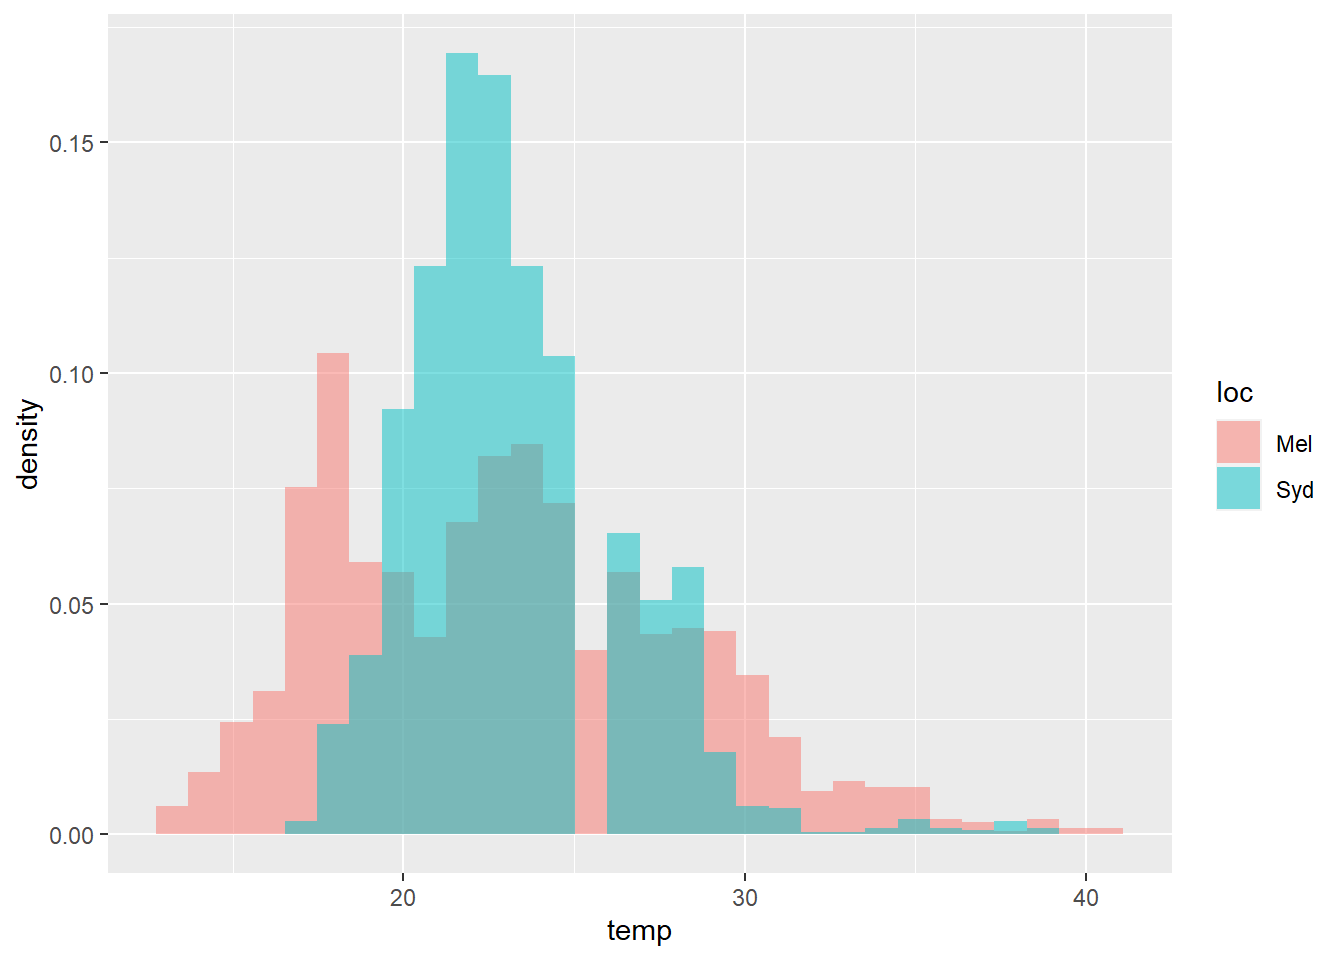
\includegraphics{template_simplified_files/figure-latex/charts-1.pdf}

\hypertarget{findings-and-conclusion}{%
\section{Findings and conclusion}\label{findings-and-conclusion}}

\textless what conclusions did you come to as a result of the analysis
of your data and of the group's data.\\
Criterion 2: Justifies the analysis of the obtained data, including
quality issues, to draw conclusions in a professional and engaging
manner.\textgreater{}

\hypertarget{discussion}{%
\section{Discussion}\label{discussion}}

\textless discuss aspects of the process that you see as important. For
example, what difficulties did you encounter; how could you avoid
problems if you did it again; etc\textgreater{}

Your `justification' and evaluation of your approach is likely to go in
this section, but may also be threaded through the preceding sections.
This includes Criterion 3: Identifies, contextualises, and reflects on
the ethical, privacy, and legal issues relevant to the collection and
analysis of personal data of self and others. \textgreater{}

\hypertarget{reflection}{%
\section{Reflection}\label{reflection}}

\textless General reflection on what you learnt during this task. What
are you unsure about? What would you do differently if you had to do it
all again?\\
Criteria 4: Connects the individual experience of this QS project to the
practice of data science (and the preceding three criteria).
\textgreater{}

\hypertarget{references}{%
\section{References}\label{references}}

\textless include any cited references, formatted in Harvard
style.\textgreater{}

\hypertarget{appendices}{%
\section{Appendices}\label{appendices}}

\textless include samples of your data - enough to give a sense of what
your raw data looks like\textgreater{}

\hypertarget{other}{%
\section{Other}\label{other}}

If you are submitting any additional materials, such as short multimedia
presentations or visualisations (such as Prezi, or voice-over
video/screen capture, etc), they probably can't be submitted through
UTSOnline so you will need to arrange some other process such as posting
on YouTube or elsewhere, or handing in a memory stick or CD/DVD. Please
ensure that additional material like this is accessible to the markers
(test this by accessing it through someone else's computer) and avoid
any restrictive or proprietary software constraints. Remember to check
any inculded web links!

Diagrams, figures, charts and illustrations must be labelled, and
explained, and must be referred to from somewhere in the report. If
drawn from another source, then the source must be provided.

\end{document}
